\documentclass[conference]{IEEEtran}
\usepackage[T1]{fontenc}
\usepackage{cite,amsmath,amssymb,booktabs,graphicx,url,xurl}
\usepackage{algorithm,algorithmic}
\usepackage{balance}
\usepackage[hidelinks]{hyperref}
\graphicspath{{figures/}{revision/figures/}}
\newcommand{\sig}{\sigma}
\newcommand{\ComparisonRows}{%
Single margin & 0.648 & 0.520 & 0.519 & 0.347 & 0.654 & 34.6 \\
Full earliest & 0.676 & 0.606 & 0.608 & 0.347 & 0.698 & 67.2 \\
Full margin & 0.676 & 0.606 & 0.608 & 0.310 & 0.698 & 69.4 \\
Full congestion & 0.674 & 0.586 & 0.596 & 0.280 & 0.698 & 77.1 \\
Full random & 0.678 & 0.599 & 0.603 & 0.315 & 0.698 & 72.8 \\
Full learned & 0.676 & 0.596 & 0.601 & 0.292 & 0.696 & 112.1 \\
RACS default & 0.676 & 0.601 & 0.606 & 0.289 & 0.697 & 75.3 \\%
}

\newcommand{\StatisticsRows}{%
Single margin & +8.11 & [1.11, 16.30] & 0.125 & 1.00 \\
Full earliest & -0.41 & [-0.96, 0.00] & 0.500 & 1.00 \\
Full margin & -0.41 & [-0.96, 0.00] & 0.500 & 1.00 \\
Full congestion & +1.52 & [0.37, 2.78] & 0.125 & 1.00 \\
Full learned & +0.52 & [-0.67, 2.22] & 1.000 & 1.00 \\
Full random & +0.29 & [-0.38, 1.04] & 0.625 & 1.00 \\%
}

\newcommand{\CalibrationRows}{%
\mbox{5, 10, 20} & 0.036 & 0.056 & 0.014 & 0.313 & 0.190 & 0.392 \\
40 & 0.167 & 0.167 & 0.167 & 0.167 & 0.167 & 0.167 \\%
}

\newcommand{\CalibratedComparisonRows}{%
RACS equal & 0.680 & 0.602 & 0.606 & 0.318 & 0.699 & 68.6 \\
RACS calibrated & 0.680 & 0.602 & 0.606 & 0.340 & 0.699 & 68.3 \\%
}

\begin{document}
\title{RACS: Reliability-Aware Congestion-Stressed Scheduling for Earth Observation in LEO Satellite Networks}
\author{\IEEEauthorblockN{K Deepak Chowdary, Rajendra Hegadi, and Suvadip Hazra}
\IEEEauthorblockA{Indian Institute of Information Technology Dharwad, India\\
deepak.24phdcs02@iiitdwd.ac.in, rajendra.hegadi@gmail.com, suvadip@iiitdwd.ac.in}}
\maketitle

\begin{abstract}
Earth-observation requests require image capture and data delivery before a deadline. This work-in-progress tests whether more delivery options or a different ranking rule improves completion. RACS combines observations from multiple satellites and divides delivery across communication windows. It can also forward data through one other satellite. Its reliability margin measures spare time and capacity, not success probability. Full-capability comparators share its options and limits. We evaluate nine synthetic instances under four stress transformations. Combined-stress completion is 60.1\% for RACS and 52.0\% for restricted single-satellite scheduling. Matched earliest/margin selection reaches 60.6\%. Gains mainly reflect flexibility. Calibrated weights match equal-weight completion; independent validation remains necessary.
\end{abstract}
\begin{IEEEkeywords}
Earth observation, LEO scheduling, downlink capacity, matched baselines, feasibility margins.
\end{IEEEkeywords}

\section{Introduction and Positioning}
An Earth-observation (EO) request requires both capture and timely delivery. A low-Earth-orbit (LEO) satellite can send data to a ground station only during a downlink contact window. If a request produces 2 GB but timely direct contacts carry only 1 GB, capture alone is insufficient. Another contact or forwarding satellite (a \emph{relay}) is needed. RACS checks capture and delivery together (Fig.~\ref{fig:system}).

Our earlier studies address visibility risk~\cite{deepak_visibility} and path selection~\cite{deepak_disagreement}. Here, we schedule both capture and delivery~\cite{ferrari}. We separate the effects of extra delivery options and the ranking rule.

Prior methods optimize capture and delivery jointly~\cite{levinson}. Others learn joint plans~\cite{li,cheng}, observation order~\cite{liu}, or search decisions~\cite{jacquet}, and consider image quality~\cite{mercado}. Our work-in-progress (WiP) isolates flexibility from scoring, without claiming superiority over these systems.

A high score cannot repair a missed contact or exhausted data storage. RACS therefore rejects infeasible plans before scoring. Among valid plans, it weighs spare time and capacity against delay and relay use. This is a preference rule, not a guarantee for later requests. The model below defines what makes a plan feasible.

\begin{figure*}[t]
\centering
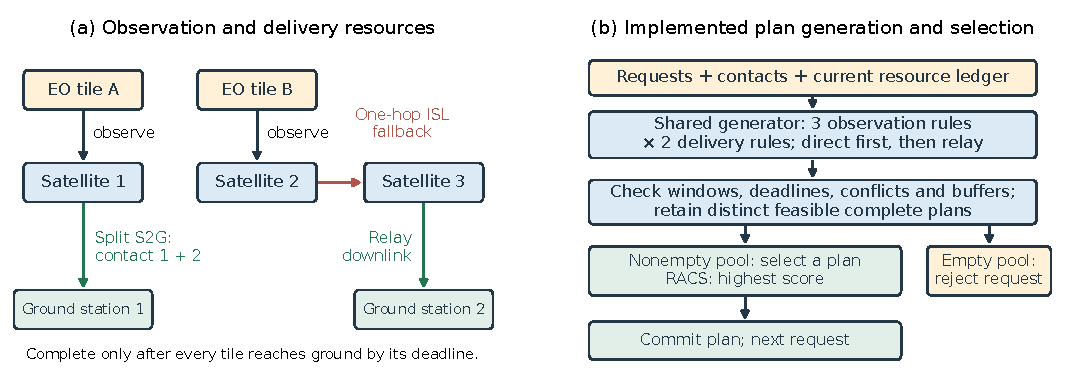
\includegraphics[width=.94\textwidth]{racs_system_and_selection.pdf}
\caption{(a) Capture and delivery paths, with illustrative geometry. (b) Every full-capability method combines three capture rules with two delivery rules to build up to six plans, checks feasibility, then selects one. Only selection differs. Single margin restricts each request to one satellite and one downlink window.}
\label{fig:system}
\end{figure*}

\section{Model and Reproducibility Scope}
\textbf{Terminology.} A \emph{request} is an EO job containing indivisible image tiles or sensing points (\emph{atomic observations}). An observation window permits capture. A satellite-to-ground (S2G) window permits delivery to a ground station. An inter-satellite link (ISL) window permits exchange between satellites. Completion requires all observations to be captured and all data delivered before the deadline.

Let $\mathcal S$ and $\mathcal G$ denote satellites and ground stations. Request $i$ has earliest start $a_i$, deadline $d_i$, importance $p_i$, and observations $\mathcal A_i$. Observation $j$ takes $\tau_j$ seconds and produces $v_j$ gigabytes (GB). A central \emph{batch} planner knows all requests in advance. Separate tiles can use different satellites; continuous single-pass imaging is outside the model.

\subsection{Contacts and resource constraints}
Input windows are fixed intervals $[b_w,e_w)$. Each observation must fit for exactly $\tau_j$ seconds. At rate $B_w$ gigabits/s, a window carries $C_w=B_w(e_w-b_w)/8$ GB. Delivery can span several windows. Each is reserved in full. A satellite or ground station handles one operation at a time, so capture, transmission, and relay cannot overlap on it.

If direct delivery fails, data may pass through one other satellite: a \emph{one-hop relay}. Moving $v$ GB at ISL rate $B^{I}$ takes $\lceil8v/B^{I}\rceil$ seconds. The link and both satellites are reserved for that time. The relay stores the data, then uses a separate S2G contact. Storage is checked whenever data arrive or leave. Transfers do not share bandwidth simultaneously. Signal travel time, turning time, battery dynamics, and packet loss are omitted.

Acceptance requires capture and delivery before $d_i$, without resource violations. We maximize completed priority, $\sum_i p_ix_i$, where $x_i=1$ means complete delivery and $0$ means rejection. The heuristic does not guarantee the maximum. Rejections are unmet demand, not measured late transmissions.

\subsection{Dataset and orbital assumptions}
The nine DataPort scenarios~\cite{dataset} start on 2024-01-01 UTC. They span 24 h with 240-s steps; the tiny case spans 6 h with 60-s steps. RACS reads supplied contacts without recomputing orbits. Their generation lacks complete documentation of the orbit method, Earth model, visibility thresholds, and timing tolerance. We test scheduling, not orbital accuracy. All methods discard observation windows too short for capture; none extends them.

All supplied observation contacts are checked within task lifetimes without fleet-size or top-$k$ cutoffs; delivery must be feasible. Future contacts are available to the batch planner. Greedy construction is not exhaustive; evaluated fleet sizes are not algorithmic limits.

\begin{table}[t]
\caption{Benchmark scope and controlled transformations.}
\label{tab:setup}\centering\footnotesize
\begin{tabular}{@{}ll@{}}\toprule
Parameter & Value or interpretation\\\midrule
Instances & 4 normal, 4 congested, 1 tiny\\
Fleet size; requests & 5--40; 5--100 per instance\\
Atomic observations & Up to 252 per instance\\
Observation / S2G windows & Up to 48,662 / 1,042\\
Planning horizon; step & 24 h; 240 s (tiny: 6 h; 60 s)\\
Deadline-only stress & $(d_i-a_i)\times0.70$\\
Bandwidth-only stress & S2G rate $\times0.65$\\
Volume-only stress & $v_j\times1.35$\\
Combined stress & Deadline $\times0.65$, rate $\times0.60$,\\
& volume $\times1.35$\\\bottomrule
\end{tabular}
\end{table}

\section{RACS Decision Rule}
RACS first checks whether a plan can finish. It then compares the valid plans. All methods order requests by shorter lifetime, higher priority, less data, then identifier: $(d_i-a_i,-p_i,\sum_jv_j,i)$. Longer atomic observations are planned first.

For each request, we try three capture rules: earliest finish, least reserved satellite time, and earliest direct-downlink finish. Each is paired with two delivery rules: time order and largest capacity first. These pairs produce at most six \emph{candidate plans} for capture and delivery. Ties use finish time and identifiers. Each plan tries direct delivery before a one-hop relay. We discard infeasible and duplicate plans, leaving the set $\mathcal Q_i^f$. This small search does not enumerate all possible schedules.

Plan $q$ delivers volume $V_i=\sum_jv_j$, reserves S2G capacity $C_q$, and finishes at $t_q$. We score its remaining time (slack $L_q$), fraction of reserved capacity used (occupancy $\rho_q$), and delay in hours ($D_q$):
\begin{gather}
L_q=d_i-t_q, \qquad \rho_q=V_i/\max(C_q,10^{-9}),\\
R_q=.55\sig(L_q/1800)+.45\sig((C_q-V_i)/2),\label{eq:margin}\\
U_q=\min(1,\rho_q)(1-R_q),\quad D_q=(t_q-a_i)/3600.
\end{gather}
The sigmoid $\sig(z)=(1+e^{-z})^{-1}$ maps to $(0,1)$. Its scales are 1800 s and 2 GB. ``Reliability-aware'' refers to margin $R_q$, not success probability. Risk proxy $U_q$ penalizes high occupancy combined with low margin; it does not estimate uncertainty. Spread $M_q$ is distinct observing satellites divided by $|\mathcal A_i|$. $N_q$ counts relay transfers. Table~\ref{tab:terms} explains each preference. The score is
\begin{align}
S_q={}&2.8R_q+.4M_q-2.2\rho_q-1.6U_q\nonumber\\
      &-.15N_q-.15D_q,\label{eq:score}\\
q_i^*={}&\arg\max_{q\in\mathcal Q_i^f}S_q.\label{eq:select}
\end{align}
Equation~\eqref{eq:select} chooses the highest-scoring feasible plan. An empty set means rejection. Priority sets request order, not plan ranking. The inherited weights and scales are heuristic choices. Section IV-C tests calibration of the six outer weights.

\begin{table}[t]
\caption{Score terms: intuition and direction of preference.}
\label{tab:terms}\centering\footnotesize
\begin{tabular}{@{}cl@{}}\toprule
Term & Meaning; score preference\\\midrule
$R_q$ & Time/capacity margin; larger\\
$M_q$ & Distinct satellites / observation count; larger\\
$\rho_q$ & Fraction of reserved delivery capacity used; smaller\\
$U_q$ & Occupancy--margin risk proxy; smaller\\
$N_q$ & Relay-transfer count; smaller\\
$D_q$ & Completion delay in hours; smaller\\\bottomrule
\end{tabular}
\end{table}

\begin{algorithm}[t]
\caption{RACS with explicit plan selection}\label{alg:racs}
\begin{algorithmic}[1]
\REQUIRE Requests, contacts, and storage limits
\STATE Initialize reservation/storage record (ledger) $\mathcal L$
\FOR{request $i$ in the common lifetime--priority order}
\STATE $\mathcal Q_i^f\gets\emptyset$
\FOR{each of six observation--delivery rule pairs}
\STATE Clone $\mathcal L$; construct observations and deliveries
\STATE Check all model constraints
\STATE If complete and feasible, add plan to $\mathcal Q_i^f$
\ENDFOR
\IF{$\mathcal Q_i^f\ne\emptyset$}
\STATE Remove duplicates; select $q_i^*$ by~\eqref{eq:select}
\STATE Commit all reservations and data events of $q_i^*$
\ELSE\STATE Reject $i$ without changing $\mathcal L$
\ENDIF
\ENDFOR
\STATE Independently validate the completed schedule
\end{algorithmic}
\end{algorithm}

Adding each checked plan preserves the modeled resource constraints; unmodeled failures remain outside this guarantee. Scaling all weights by $c>0$ leaves rankings unchanged. We therefore search nonnegative weights summing to one. We next compare completion and runtime, then test weight calibration.

\section{Evaluation and Attribution}
\begin{figure*}[t]
\centering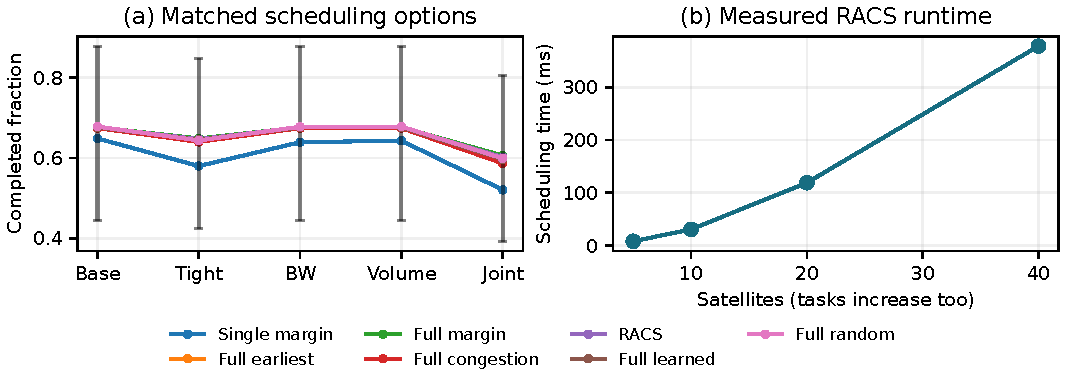
\includegraphics[width=.90\textwidth]{matched_results.pdf}
\caption{(a) Completion with matched capabilities. Base: unchanged; Tight: shorter deadlines; BW: lower bandwidth; Volume: more data; Joint: combined stress (Table~\ref{tab:setup}). Error bars show bootstrap 95\% confidence intervals for default RACS. (b) Scheduling runtime; requests and contacts also increase with fleet size. Parsing, training, and validation are excluded.}
\label{fig:results}
\end{figure*}
\subsection{Matched policies and protocol}
To isolate ranking, full-capability methods share the generator, request order, and constraints. Earliest minimizes completion time. Margin maximizes $R_q$, and congestion minimizes $\rho_q$. Random samples uniformly; learned predicts reward; RACS maximizes~\eqref{eq:score}. Earlier choices can change later candidate sets. Single margin permits one satellite/downlink. Its comparison tests restricted delivery options, not ranking alone.

The learned comparator tests data-driven rather than hand-designed ranking. It is a random forest, an ensemble of decision trees~\cite{breiman}: 64 trees, depth 5, minimum leaf 5, seed 2026. Inputs are the score features, data volume, reservation hours, and downlink count. Targets sum priority for the current and next three requests under simulated earliest-plan decisions (a \emph{rollout}). Training uses other fleet sizes' base instances, excluding the test size.

Each scenario runs unchanged (\emph{base}) and under Table~\ref{tab:setup}'s artificial stresses. Random seeds 0--9 are averaged within scenario. For request set $\mathcal T$, completion is $\sum_i x_i/|\mathcal T|$. Priority reward is $\sum_i p_ix_i/\sum_i p_i$; miss is one minus completion. We average scenario ratios rather than pool requests. Classes $\mathcal C$ group priorities 1--3, 4--6, and 7--10, excluding empty classes. Let $r_c$ be each class's completion rate. Jain fairness~\cite{jain}, $(\sum_c r_c)^2/(|\mathcal C|\sum_c r_c^2)$, measures their balance. Lower occupancy leaves more reserved capacity unused, not necessarily greater efficiency.

\begin{table}[t]
\caption{Matched results. Compl.: completion fraction; Reward: completed-priority fraction; $\rho$: capacity occupancy; Jain: priority-class fairness; ms: scheduling runtime in milliseconds.}
\label{tab:results}\centering\footnotesize
\setlength{\tabcolsep}{3pt}
\begin{tabular}{@{}lrrrrrr@{}}\toprule
& Base & \multicolumn{5}{c}{Combined stress}\\
\cmidrule(lr){2-2}\cmidrule(lr){3-7}
Policy & Compl. & Compl. & Reward & $\rho$ & Jain & ms\\\midrule
\ComparisonRows
\CalibratedComparisonRows
\bottomrule\end{tabular}
\end{table}

\subsection{Results and statistical evidence}
The matched comparisons attribute the main gain to delivery flexibility rather than the ranking score.
Under combined stress, RACS completes 8.11 percentage points more requests than single margin and 0.52 more than learned (Table~\ref{tab:results}). It trails full earliest/margin by 0.41 points. Base completion matches earliest, margin, and learned; random is slightly higher. Occupancy falls from earliest's 0.347 to 0.289, leaving more reserved capacity unused. This is a trade-off, not evidence of better completion or reduced network congestion.

Jain fairness improves over single margin, not full earliest (Table~\ref{tab:results}); uniformly poor service can also be fair.

Paired bootstrap intervals use 10,000 resamples of nine scenarios~\cite{efron}. Exact Wilcoxon tests omit zero differences and average tied ranks~\cite{wilcoxon}. Holm correction covers 30 completion comparisons~\cite{holm}; none establishes RACS superiority. Stress variants are not independent deployments.

\begin{table}[t]
\caption{Selected normalized weights. Grouped sizes were held out separately with all their variants.}
\label{tab:weights}\centering\footnotesize
\setlength{\tabcolsep}{3pt}
\begin{tabular}{@{}lrrrrrr@{}}\toprule
Held out & $w_R$ & $w_M$ & $w_\rho$ & $w_U$ & $w_N$ & $w_D$\\\midrule
\CalibrationRows
\bottomrule\end{tabular}
\end{table}

\subsection{Weight evidence and optimization check}
We next ask whether tuning the weights improves these results. The weights are tunable coefficients (\emph{hyperparameters}), not physical constants. We exclude fleet group $g$ and all its variants from tuning~\cite{cawley}, then select
\begin{equation}
w^*_{-g}=\arg\max_{w\in\mathcal W}\frac{\sum_{h\in\mathcal F\setminus\{g\}}\overline J_h(w)}{|\mathcal F|-1},
\end{equation}
Here $\mathcal F$ contains fleet-size groups. $\overline J_h$ is mean completed-priority fraction in group $h$. We test 33 weight vectors in $\mathcal W$: normalized default, equal, and 31 Dirichlet$(1)$ random draws (seed 20261003). Candidate order breaks ties. Table~\ref{tab:weights} lists the selection for each excluded group.

We average fleet groups equally. Calibration increases completion by 0.258 percentage points and reward by 0.191 over default. Equal coefficients achieve the same results. Neither gain is significant: raw $p=0.5$, Holm $p_H=1$. Eight tests cover two metrics and four comparators. Intervals resample four groups. Training sets overlap, and the benchmark was previously inspected. These results are therefore exploratory.

The score permits different preferences, not just completion maximization. Equal and calibrated weights yield equal completion but different occupancy (Table~\ref{tab:results}). Tuning is not demonstrably necessary or superior here.

All 1,980 schedules pass validation. Removing spread raises mean completion by 0.148 points; removing relay penalty lowers it by 0.259. Some terms may therefore be unnecessary. Earlier 315 sensitivity runs gave combined completion 0.5933--0.6037. These tests assess sensitivity, not weight optimality.

The 40-satellite run takes 378 ms in Python 3.11.5 on ARM macOS (Fig.~\ref{fig:results}). Single-run timings include construction/selection, not parsing, training, or validation. A mixed-integer linear program (MILP) optimizes a fixed plan pool under resource/storage limits. On the largest normal case under combined stress, optimal priority is 339 versus greedy's 210. This certifies only that pool, not RACS's changing plans.

\section{Conclusion and Future Work}
Next, we will test fewer score terms and document contacts before assessing EOS-Bench~\cite{eosbench}, AEOS-Bench~\cite{aeosbench}, and CelesTrak-derived inputs~\cite{celestrak}. Operational scheduling requires slew-rate limits (camera turning time) and battery constraints. External validation remains pending; orbit-derived contacts are still simulated. Repository: \url{https://github.com/KarusalaDeepak/leo-eo-scheduling}.

\begin{thebibliography}{19}
\bibitem{deepak_visibility} K. Deepak Chowdary, S. Hazra, and R. Hegadi, ``Risk-aware evaluation of LEO satellite visibility windows using survival analysis,'' manuscript, 2026.
\bibitem{deepak_disagreement} K. Deepak Chowdary, S. Hazra, R. Hegadi, and Chinmayananda A, ``Delay-aware disagreement diagnostics and evidence-gated 5G--LEO multi-access path selection,'' manuscript, 2026.
\bibitem{ferrari} B. Ferrari, J.-F. Cordeau, M. Delorme, M. Iori, and R. Orosei, ``Satellite scheduling problems: A survey of applications in Earth and outer space observation,'' \emph{Computers \& Operations Research}, vol. 173, art. 106875, 2025, doi: 10.1016/j.cor.2024.106875.
\bibitem{levinson} R. Levinson, V. Ravindra, and S. Roy-Singh, ``Optimal planning to coordinate science data collection and downlink for a constellation of agile satellites with limited storage,'' in \emph{Proc. IJCAI}, 2025, pp. 8544--8553, doi: 10.24963/ijcai.2025/950.
\bibitem{li} P. Li, H. Wang, Y. Zhang, and R. Pan, ``Mission planning for distributed multiple agile Earth observing satellites by attention-based deep reinforcement learning method,'' \emph{Advances in Space Research}, vol. 74, no. 5, pp. 2388--2404, 2024, doi: 10.1016/j.asr.2024.06.003.
\bibitem{cheng} J. Cheng \emph{et al.}, ``UHTS-DRL: A deep reinforcement learning framework for integrated agile satellite observation and data transmission scheduling,'' \emph{Information Sciences}, vol. 740, art. 123200, 2026, doi: 10.1016/j.ins.2026.123200.
\bibitem{liu} Z. Liu, W. Xiong, Z. Jia, and C. Han, ``Two-stage deep reinforcement learning method for agile optical satellite scheduling problem,'' \emph{Complex \& Intelligent Systems}, vol. 11, art. 35, 2025, doi: 10.1007/s40747-024-01667-x.
\bibitem{jacquet} A. Jacquet, G. Infantes, E. Benazera, V. Baudoui, J. Guerra, and S. Roussel, ``Earth observation satellite scheduling with graph neural networks and Monte Carlo tree search,'' \emph{IWPSS}, 2025, arXiv:2408.15041v2.
\bibitem{mercado} A. M. Mercado-Martinez, B. Soret, and A. Jurado-Navas, ``An energy-efficient learning solution for the agile Earth observation satellite scheduling problem,'' arXiv:2503.04803, 2025.
\bibitem{dataset} IEEE DataPort, ``Congestion-stressed LEO satellite network dataset for Earth observation task scheduling and routing,'' dataset, 2026. [Online]. Available: \url{https://ieee-dataport.org/documents/congestion-stressed-leo-satellite-network-dataset-earth-observation-task-scheduling-and}
\bibitem{breiman} L. Breiman, ``Random forests,'' \emph{Machine Learning}, vol. 45, pp. 5--32, 2001, doi: 10.1023/A:1010933404324.
\bibitem{jain} R. Jain, D.-M. Chiu, and W. Hawe, ``A quantitative measure of fairness and discrimination for resource allocation in shared computer systems,'' DEC Research Report TR-301, 1984.
\bibitem{efron} B. Efron, ``Bootstrap methods: Another look at the jackknife,'' \emph{Annals of Statistics}, vol. 7, no. 1, pp. 1--26, 1979, doi: 10.1214/aos/1176344552.
\bibitem{wilcoxon} F. Wilcoxon, ``Individual comparisons by ranking methods,'' \emph{Biometrics Bulletin}, vol. 1, no. 6, pp. 80--83, 1945, doi: 10.2307/3001968.
\bibitem{holm} S. Holm, ``A simple sequentially rejective multiple test procedure,'' \emph{Scandinavian Journal of Statistics}, vol. 6, no. 2, pp. 65--70, 1979.
\bibitem{cawley} G. C. Cawley and N. L. C. Talbot, ``On over-fitting in model selection and subsequent selection bias in performance evaluation,'' \emph{J. Mach. Learn. Res.}, vol. 11, pp. 2079--2107, 2010.
\bibitem{eosbench} Q. Yin \emph{et al.}, ``EOS-Bench: A comprehensive benchmark for Earth observation satellite scheduling,'' arXiv:2604.25782, 2026.
\bibitem{aeosbench} L. Wang \emph{et al.}, ``Towards realistic Earth-observation constellation scheduling: Benchmark and methodology,'' arXiv:2510.26297, 2025.
\bibitem{celestrak} CelesTrak, ``Current GP element sets.'' [Online]. Available: \url{https://celestrak.org/NORAD/elements/}. Accessed: Oct. 3, 2026.
\end{thebibliography}
\end{document}
